\documentclass[a4paper]{llncs}
\usepackage{amsmath, amssymb}
\usepackage{makeidx}  % allows for indexgeneration
\usepackage[pdftex]{graphicx} % PNGs
\usepackage[ngerman,english]{babel}
\usepackage[utf8x]{inputenc}
\usepackage[T1]{fontenc}
\usepackage{listings} % for sourcecode
\usepackage{graphviz} % graphs
\usepackage{array} % tables
\usepackage{afterpage} % figures
\usepackage{float} % figures

%Smalltalk listings
\lstdefinelanguage{Smalltalk}{
  morekeywords={true,false,self,super,nil},
  sensitive=true,
  morecomment=[s]{"}{"},
  morestring=[d]',
  style=SmalltalkStyle
}
\lstdefinestyle{SmalltalkStyle}{
  %literate={:=}{{$\gets$}}1{^}{{$\uparrow$}}1{>>}{{\frqq}}1
  literate={^}{{$\uparrow$}}1{>>}{{\frqq}}1
}
\lstset{%
  	language=Smalltalk,
	basicstyle=\small,
	frame=single
}

% Ein beispiel Listing
%
%\begin{lstlisting}[language=Smalltalk]
%HelloWorld>>sayHelloTo: aString
%    "print a hello world message"
%    Transcript show: 'Hello, ', aString, '!'
%    name := 'a new name' "This is a comment"
%    ^ name
%\end{lstlisting}


\begin{document}
\mainmatter              % start of the contributions
\title{XO-Bubbles}
\subtitle{A Frozen Bubble Clone in Smalltalk/Squeak}
\date{\today}
\author{Tim Felgentreff, 738147}
\author{Konstantin Haase\inst{1}, Tim Felgentreff\inst{1}, Johannes Wollert\inst{1}, 
Michael Winkelmann\inst{2}, Robert Pfeiffer\inst{1}}

\institute{%
Hasso-Plattner-Institut, Universität Potsdam, D-14482 Potsdam, Germany,\\
\email{\{konstantin.haase,tim.felgentreff,johannes.wollert, robert.pfeiffer\}@student.hpi.uni-potsdam.de}
\and
Institut für Informatik, Universität Potsdam, D-14482 Potsdam, Germany,\\
\email{mwinkel@uni-potsdam.de}}

\maketitle

\begin{abstract}
  {With the rise of the Web 2.0 social networking sites, our social interactions
have gained another facet. As with every social activity, confinement
to a lone computer session thins out the user-group considerably.
If the social web is 
to persists this cannot be the end of the story. Yet, broad use of social networks on-the-go 
with the help of
the increasingly popular smartphones is held back by the large form factor of 
those devices, and the fact that they are not specialized to perform this 
task. In this paper, we propose a tiny mobile device tailored to the needs 
of the social web user. In our user study, participants were able to access
their most wanted features more quickly and with less error compared to a 
regular smartphone with a web browser.
}
\end{abstract}

%:= the shortest path between a commonly believed fact
%and the research question you are answering in your paper
%
%Example (Shift, CHI 2007)
%to save time for retrieving the stylus, users operate PDAs using touch
%finger tip size and occlusion make acquisition of small targets hard
% zooming does not fix that occlusion (see section “user test paper”)
% offset cursor solves the problem, but has three drawbacks
%we propose ‘Shift’. It solves the problem while avoiding the 3 drawbacks
%
%one paragraph for each logical step in that argument
%if you need more than, say, 6 paragraphs you are probably underestimating your audience and started too far back
%write in logical order, not in the chronological order in which you came up with it (this is not a diary)
%
\section{Introduction}
Social Web is the next logical extension to Mail and SMS to keep track of your associates. 
Social websites have gained much larger user bases than ``traditional'' web communities and demand
for new ways of access to the communities is high.
Traditionally, 
anything web-related was performed at a computer and only recently, with the wide-spread adoption of 
smartphones, the desire to use such networks ubiquitously emerged. Let's see how this is done today:
\begin{itemize}
  \item %
    Users usually 
    use the web browser of their smartphone system. This is the obvious solution for the inexperienced,
    and it is guaranteed to work with their social network of choice.
  \item Even with clever zooming techniques, the small screen is unsuitable for feature-packed sites such as Facebook\registered. 
    This alienates users. Still, they will likely not give up social networking, but rather look for a new 
    way of using it on-the-go
  \item Persistent users will soon find specialized apps for example on the Android\trademark platform or for the 
    Palm\registered Pre, however, 
    those apps still have to be started each time. Such delay, now matter how small, may offset users from doing what they were 
    trying to do completely, as users generally do not see the point of waiting 10 seconds for an application to start 
    only to see they do not have any new messages in their inbox.
\end{itemize}
To resolve those issues,we propose a specialized, small and unobtrusive device tailored towards a 
single purpose: to access the 
most used features of social networks in a consistent manner without delay or other 
inconvenience. We want social networking to
become the natural daily experience its users wanted it to be all along.
\begin{figure}[h]
  \begin{center}
    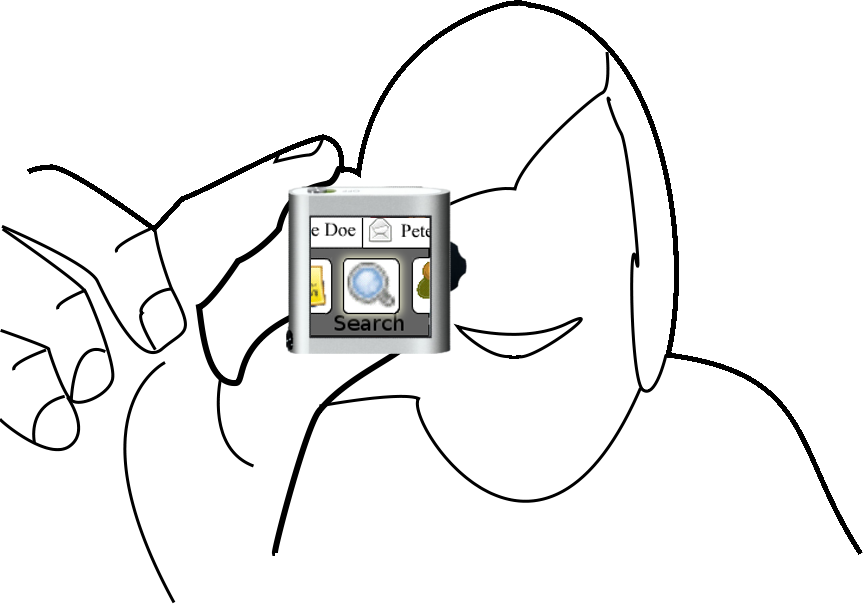
\includegraphics[width=0.8\linewidth]{imgs/main.png}
  \end{center}
  \caption{The SocioPath Device in Context}
  \label{fig:main}
\end{figure}

\input{problem_domain}
\section{Architecture}
In our system we have a set of classes which are central to the 
game. Those classes handle theming, player actions, game logic 
and the graphical representation of the game. These central
classes of our game are depicted in Fig.\ref{fig:architecture}.
%
The first instantiated class is FBGame. FBGame controls the game functionality, 
like the number of players, reward strategies like highscores and the
conditions of victory and defeat. FBGame is also responsible for instantiating
the FBWorld class which encapsulates graphical representation of the game.

FBWorld is passed a symbol at startup, which is resolved to a FBTheme. FBWorld 
holds a reference to the current theme and creates its main submorphs, like
a menu, highscore list the changing backgrounds and the in-game playfields.
These Morphs, however, are not held in an instance variable of any kind, but 
are returned to the FBGame instance, for co-ordination.\\
Out of technical necessity, FBWorld also catches all keytrokes, handling them, 
however, is up to the FBGame. Global events, like pause and quit, are handled 
directly, all other keystrokes are passed on to all playfields in the game (if any)
and handled there.

FBPlayfields are created by the world upon the requirements of the theme
and then returned to the FBGame. The playfields receive their own reference 
to the theme and are themselves responsible for their content and reaction on 
player input, thus allowing us to implement multiplayer gaming simply by creating 
more playfields in our world.
%
\begin{figure}[bt]
  \begin{center}
    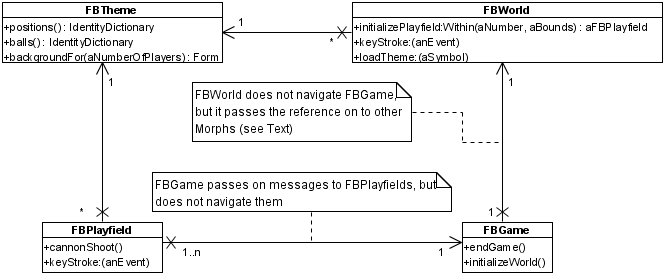
\includegraphics[width=0.6\linewidth]{images/architecture.png}
  \end{center}
  \caption{The central system architecture}
  \label{fig:architecture}
\end{figure}



\section{Design Process}
\subsection{Design Goals}
In order to achieve a pleasant and cleanly written FrozenBubble clone, we specified certain design goals.
A goal we set for ourselves very early was themeability, e.g. the ability to modify and 
adjust certain visual and logical aspects of the game (for example ball images or 
cannon positions). This demands an efficient and maintainable theme management 
system, as lots of pictures and data need to be processed.
As previously stated, another important aspect of our clone is ''realistic'' 
collision between objects, which came with certain performance considerations.
Lastly, we wanted our game to support multiplayer functionality. Given the time 
needed to implement networking, we decided to focus on a local multiplayer modes. 

\subsection{Slow Disk I/O}
%
Different from the original, we wanted to decouple the game from its representation 
to the point that we could allow different themes to change the positions of the 
game objects for different images and backgrounds. We decided to use png images to allow 
great visual flexibility and XML files to define the theme's positions. As disk I/O
is expensive, we needed a way to avoid it as much as possible, without sacrificing 
flexibility. Thus, lazy initialization for our FBTheme class was not an option. 
We created a class solely responsible for caching images and use the flyweight 
pattern to avoid reloading a theme we already loaded.
%
\subsection{Collision Between Balls}
\label{sec:collision}
When a ball is shot into the playfield, it has to interact with the plafield 
and other objects in its path. Simply looping over all those objects and 
testing for collision is in O(n) and result in slower 
movement of the ball and a general loss in responsiveness. A quick solution 
would have been to keep two lists of all objects sorted by their x and by their 
y axis, and only testing those items closest to the current ball in both lists.
Now O(n) would only be the worst case. 
It occured to us that using rasterization or using precalculated vectors similar 
to ray-tracing techniques could get us a constant complexity. We decided 
to implement rasterization, because it was a faster solution and allowed straight 
forward optimization.
%
\subsection{Falling Balls}
\label{sec:garbage}
When balls can collide and stick to each other, having them fall down 
if three or more of the same kind touch is trivial. However, balls 
hanging off balls that fall may have to fall as well. We considered 
two ways of checking for such conditions. We first planned to regard balls in the 
playfield as a network of nodes and use a graph search algorithm to determine 
whether or not a given ball has a connection to the top of the playfield via 
others. This proved difficult to implement and hurting encapsulation. Thus 
<<<<<<< HEAD:design.tex
we applied a metaphor of a garbage collector (GC) to the problem, where balls
ball that are not connected to the top are collected. Performance was no pressing 
concern here, as the number of balls in one playfield is relatively limited, 
and the algorithm runs at a moment where the user has just shot, so taking a second 
for the calculation would not hurt the game flow.
=======
we applied a metaphor of a garbage collector (GC) to the problem. First we used a
``reference counting GC'' where a ball registered itself with the balls he hung 
off. If any those balls fell, they reported to each registree so that they would 
decrement their reference count. If the reference count fell to zero, the ball 
would fall. However, this approach led to some problems with circular shapes 
in the playfield. Due to this we switched to a ``mark and sweep GC'' which traverses
over the balls in the field. Though this might sound less optimal performance-wise,
you have to keep in mind that the number of balls in one playfield is relatively limited, 
and also that the GC runs at a moment where the user cannot shoot anyway, so 
it is not time-critical.

\subsection{Simple Multiplayer Mode}
Several problems occured when we implemented a simple local multiplayer mode. In this chapter, 
we will discuss the most important design decissions.

%
  \paragraph{Players need to be informed of critical actions happening in other players' playfields}
    Direct communication between playfields would be the most simple solution like and 
    could be implemented easily. Additionally only the most rudimentary communication is needed,
    so there would be very few overhead. But this is not an object-oriented solution and playfields 
    would need to be hardcodedly enumerated, making the code hardly maintainable and badly extensible.\\
    In contrast, delegating communication through a mediator makes very maintainable and
    expandable code. Other than the previous proposal, this is indeed an object-oriented 
    take on the problem. However, there is more than twice as much communication happening 
    compared to the previous, simplified solution.\\
    Due to the obvious disadvantages of hardcoding different playfields, we chose the latter proposal.\\

  \paragraph{Different playfields have to be controlled by different players.
             And, of course, different playfields have to exist in the first place.}
    Our first idea we came up with was enabling the generic playfield to manage all needed behaviour
    on itself. That way, no new code needs to be introduced, rendering this scheme very simple.
    On the other hand, the playfield might have to be extended for all purposes to work properly. 
    This might lead to a very huge class indeed, affecting the readability.\\
    Introducing an Abstract Factory for playfields was another idea, thus implementing several 
    behavioural patterns. The obvious advantage of this proposal is, that Abstract Factories 
    are extensible and object-oriented. The downside of it would be, that this is a very powerful 
    pattern and would probably be overindulgence because we just need two different playfields 
    (single- and multiplayer behaviour). Because of that, we chose our initial idea of keeping 
    things simple.\\
%
\end{description}
%


\section{Development Process}
Our development roadmap scheduled three successive releases. The first release, called ``Waitaha'', was developed using the pair programming technique: While one developer was typing code at least one other developer was constantly watching and reviewing it. This version was the first basic clone of the original Frozen Bubble game.

``Little Blue'' was the second release and the first one to be presented to the public, featuring a restructered architecture and a stable API. With this version there was a shift in development with each of the developers encountered a shift in programming techniques: Less pair programming but heavy reliance on version control (Monticello and Git) and frequent meetings for code review.

The final version - ``Rockhopper'' - is considered feature complete and has no known bug\footnote{at the time of writing}.
\section{Conclusions}
We managed to build a functional and flexible FrozenBubble clone for Morphic,
but given our time constraints, not all features we would have liked to implement
made it into the final version. Especially a working network multiplayer mode would
have been quite delightful. It is possible however to play a local multiplayer mode,
limited in use only by the self-blocking keypress messages provided by morphic.

\section*{Acknowledgements}
We are indebted to the developers of Frozen Bubble for allowing us to release 
our clone with the name and graphics of the original game under the MIT 
license. We also thank Professor Hirschfeld, Tobias Pape and Michael Perscheid for 
their advice.



\bibliographystyle{splncs}
\bibliography{swa}
\clearpage
\end{document}

